\documentclass[conference, a4paper]{IEEEtran}
\usepackage[utf8]{inputenc}
\usepackage[T1]{fontenc}
\usepackage{graphicx}
\usepackage{booktabs}
\usepackage[breaklinks=true]{hyperref}
\usepackage{cite}

% Evitar que el texto se salga de los margenes
\sloppy

\title{Sistema de Clasificaci\'on de Intenciones para un Asistente Virtual de Tr\'amites Universitarios}

\author{
    \IEEEauthorblockN{Equipo 7}
    \IEEEauthorblockA{Gonzalo Nahuel Acosta Lopez, Cesar Pietro Barrios Calathaki\\
    Departamento de Inform\'atica, FaCENA -- UNNE\\
    Corrientes, Argentina\\
    \texttt{gonzalineritolol@gmail.com}, \texttt{pietrocalathaki@gmail.com}}
}

\begin{document}

\maketitle

\begin{abstract}
Este trabajo presenta el desarrollo de un asistente virtual conversacional 
para orientar a estudiantes de la FaCENA-UNNE en el tr\'amite del T\'itulo 
Intermedio de Pregrado. Se implementaron y compararon tres modelos de 
clasificaci\'on de intenciones: Naive Bayes Multinomial con TF-IDF, SVM 
Lineal con TF-IDF y SVM con kernel RBF utilizando embeddings sem\'anticos 
(SentenceTransformer). El modelo ganador alcanz\'o un 81.25\% de exactitud 
y 0.81 de F1-macro, validado con 5-fold cross-validation. Se desarroll\'o 
una interfaz web funcional con Streamlit para su uso por la comunidad 
estudiantil.
\end{abstract}

\section{Introducci\'on}

\subsection{Problema y Contexto}

Los estudiantes de la UNNE que cursan carreras en la Facultad de Ciencias 
Exactas y Naturales y Agrimensura (FaCENA) enfrentan dificultades para 
comprender el proceso de obtenci\'on del T\'itulo Intermedio de Pregrado. 
El tr\'amite involucra dos etapas con requisitos y plazos espec\'{\i}ficos 
que generan consultas recurrentes a la Direcci\'on de Gesti\'on de Estudios. 
Actualmente no existe un canal automatizado que resuelva estas consultas 
de forma inmediata.

\subsection{Alcance}

El sistema desarrollado es un asistente virtual capaz de interpretar 
preguntas en lenguaje natural y clasificarlas en 16 categor\'{\i}as 
(15 intenciones del tr\'amite + fallback). Responde con informaci\'on 
oficial basada en la resoluci\'on RES-2025-7936-REC-UNNE.

\subsection{Tema Disciplinar}

Este trabajo se enmarca en Procesamiento de Lenguaje Natural (NLP), 
espec\'{\i}ficamente en clasificaci\'on de textos cortos en el dominio 
administrativo-universitario.

\subsection{Evoluci\'on respecto a la Asignatura}

Este trabajo se bas\'o en la prueba de un modelo no explorado durante 
la asignatura: SVM (M\'aquinas de Vectores de Soporte), adem\'as de 
aplicar herramientas nuevas relacionadas con el Procesamiento de 
Lenguaje Natural (PLN) como TF-IDF (modelos 1 y 2) y Embeddings 
sem\'anticos (modelo 3).

\section{M\'etodo}

\subsection{Metodolog\'{\i}a}

Se adopt\'o un proceso iterativo basado en CRISP-DM adaptado para 
aprendizaje supervisado: 1) an\'alisis del tr\'amite y relevamiento de 
consultas, 2) curado y expansi\'on del dataset con limpieza de texto, 
3) modelado con tres arquitecturas de clasificaci\'on, y 4) evaluaci\'on 
con exactitud, F1-macro, 5-fold CV y GridSearchCV.

\subsection{Modelos de IA}

Se implementaron tres modelos supervisados de clasificaci\'on multiclase 
(Tabla~\ref{tab:modelos}).

\begin{table}[h!]
\centering
\caption{Arquitecturas de los modelos implementados.}
\label{tab:modelos}
\resizebox{\columnwidth}{!}{%
\begin{tabular}{@{}lll@{}}
\toprule
\textbf{Modelo} & \textbf{Vectorizaci\'on} & \textbf{Hiperpar\'ametros} \\
\midrule
M1: MultinomialNB & TF-IDF (unigramas) & $\alpha = 0.5$ \\
M2: SVM Lineal & TF-IDF (unigramas) & $C = 1.0$, kernel = linear \\
M3: SVM RBF & SentenceTransformer (512-d) & $C = 10.0$, $\gamma$ = scale \\
\bottomrule
\end{tabular}
}
\end{table}

M1 utiliza Naive Bayes Multinomial con suavizado de Laplace ($\alpha=0.5$), 
que modela la probabilidad condicional de cada t\'ermino dada una clase. 
M2 emplea SVM lineal encontrando el hiperplano de separaci\'on \'optimo. 
M3 utiliza SVM con kernel RBF sobre embeddings sem\'anticos densos 
generados por \texttt{distiluse-base-multilingual-cased-v2}, capturando 
relaciones sem\'anticas entre las consultas.

\subsection{Experimentaci\'on}

El dataset de 240 preguntas (16 por cada una de 15 intenciones) se 
dividi\'o en 80\% entrenamiento y 20\% prueba (192/48), estratificado. 
Se realizaron tres fases experimentales: preprocesamiento (stemming, 
n-gramas, max features), optimizaci\'on (GridSearchCV + 5-fold CV), 
y validaci\'on final (entrenamiento completo + prueba cualitativa).

\section{Herramientas}

El sistema se desarroll\'o en Python 3.12. Las librer\'{\i}as principales 
se detallan en la Tabla~\ref{tab:herramientas}.

\begin{table}[h!]
\centering
\caption{Librer\'{\i}as y herramientas utilizadas.}
\label{tab:herramientas}
\resizebox{\columnwidth}{!}{%
\begin{tabular}{@{}lll@{}}
\toprule
\textbf{Librer\'{\i}a} & \textbf{Versi\'on} & \textbf{Prop\'osito} \\
\midrule
scikit-learn & 1.6 & Modelos (MultinomialNB, SVC), TfidfVectorizer, GridSearchCV \\
sentence-transformers & 3.4 & Embeddings sem\'anticos multiling\"ues \\
pandas / numpy & 2.2 / 2.0 & Manipulaci\'on de datos \\
joblib & 1.4 & Persistencia de modelos \\
streamlit & 1.57 & Interfaz web \\
\bottomrule
\end{tabular}
}
\end{table}

\section{Resultados}

\subsection{Preprocesamiento}

La Tabla~\ref{tab:preproc} muestra el impacto de distintas t\'ecnicas.

\begin{table}[h!]
\centering
\caption{Experimentos de preprocesamiento (exactitud sobre test).}
\label{tab:preproc}
\resizebox{\columnwidth}{!}{%
\begin{tabular}{@{}lccc@{}}
\toprule
\textbf{Experimento} & \textbf{NB+TF-IDF} & \textbf{SVM+TF-IDF} & \textbf{SVM+Emb.} \\
\midrule
Baseline & 77.08\% & 72.92\% & 81.25\% \\
Con stemming & 79.17\% & 70.83\% & 68.75\% \\
Bigramas (1,2) & 75.00\% & 72.92\% & --- \\
\bottomrule
\end{tabular}
}
\end{table}

El stemming beneficia a NB (+2.09\%) pero degrada los modelos con 
embeddings ($-12.5$ pp). Los unigramas superan a los bigramas por 
menor dispersi\'on con 240 muestras.

\subsection{Optimizaci\'on}

La Tabla~\ref{tab:grid} muestra los resultados de GridSearchCV.

\begin{table}[h!]
\centering
\caption{Resultados de GridSearchCV con 5-fold CV.}
\label{tab:grid}
\resizebox{\columnwidth}{!}{%
\begin{tabular}{@{}lcc@{}}
\toprule
\textbf{Modelo} & \textbf{Mejores params} & \textbf{CV F1-macro} \\
\midrule
MultinomialNB & $\alpha = 0.5$ & 0.7063 \\
SVM Lineal & $C = 1.0$ & 0.6872 \\
SVM RBF & $C = 10.0$, $\gamma$ = scale & \textbf{0.7600} \\
\bottomrule
\end{tabular}
}
\end{table}

\subsection{Resultados Finales}

La Tabla~\ref{tab:final} resume el desempe\~no final de los tres modelos.

\begin{table}[h!]
\centering
\caption{Resultados finales sobre el conjunto de prueba.}
\label{tab:final}
\resizebox{\columnwidth}{!}{%
\begin{tabular}{@{}lccc@{}}
\toprule
\textbf{Modelo} & \textbf{Exactitud} & \textbf{F1-macro} & \textbf{F1-pond.} \\
\midrule
NB + TF-IDF ($\alpha=0.5$) & 79.17\% & 0.77 & 0.79 \\
SVM Lineal + TF-IDF ($C=1.0$) & 75.00\% & 0.73 & 0.74 \\
SVM RBF + Embeddings ($C=10.0$) & \textbf{81.25\%} & \textbf{0.81} & \textbf{0.81} \\
\bottomrule
\end{tabular}
}
\end{table}

El modelo SVM con embeddings (M3) obtuvo el mejor desempe\~no. En una 
prueba cualitativa con 7 preguntas no incluidas en el dataset, clasific\'o 
6 de 7 correctamente (85.71\%).

La Figura~\ref{fig:comparison} muestra la comparaci\'on de exactitud 
entre los tres modelos, y la Figura~\ref{fig:confusion} presenta las 
matrices de confusi\'on correspondientes.

\begin{figure*}[ht]
\centering
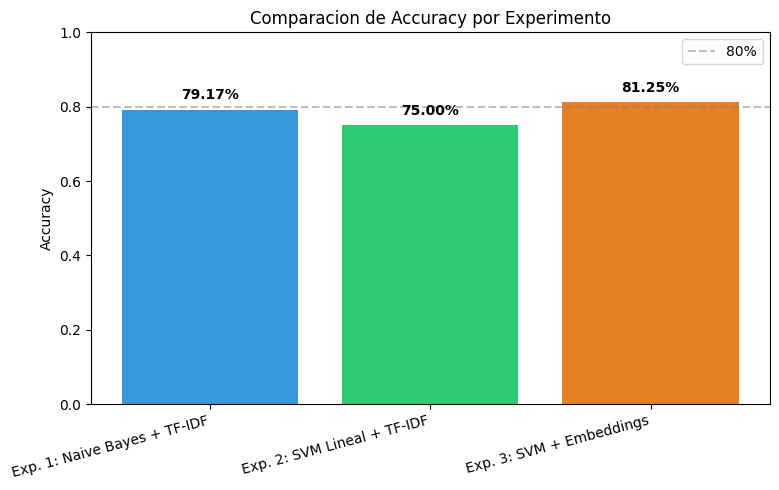
\includegraphics[width=0.72\textwidth]{img/comparison_accuracy.png}
\caption{Comparaci\'on de exactitud entre los tres modelos.}
\label{fig:comparison}
\end{figure*}

\begin{figure*}[ht]
\centering
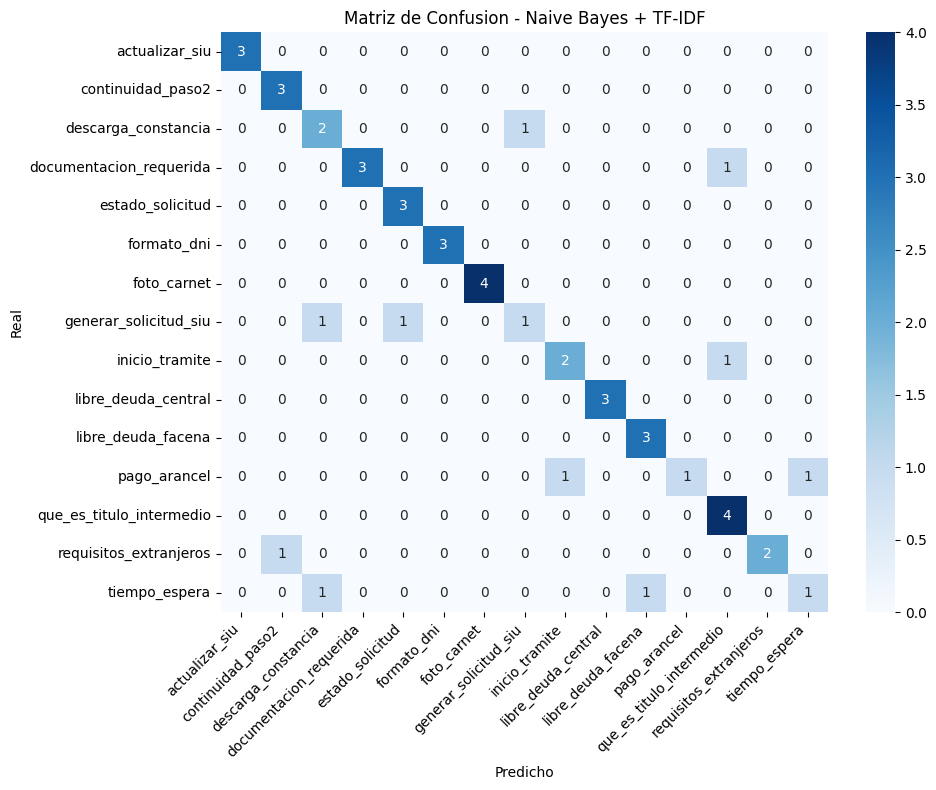
\includegraphics[width=0.30\textwidth]{img/confusion_nb.png}
\hfill
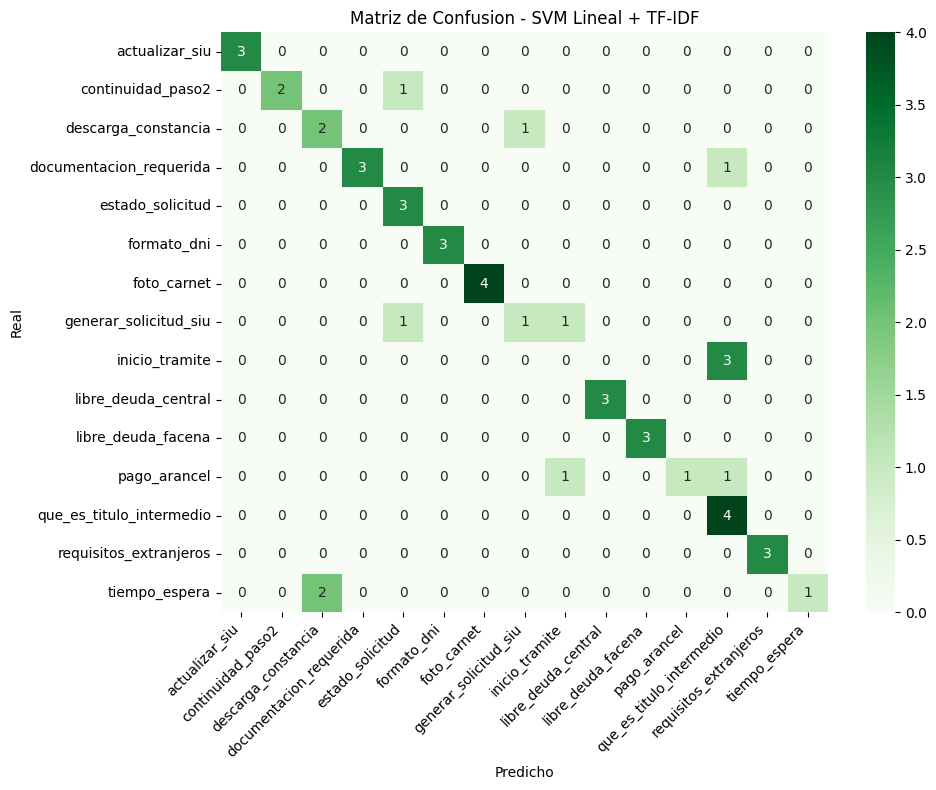
\includegraphics[width=0.30\textwidth]{img/confusion_svm_linear.png}
\hfill
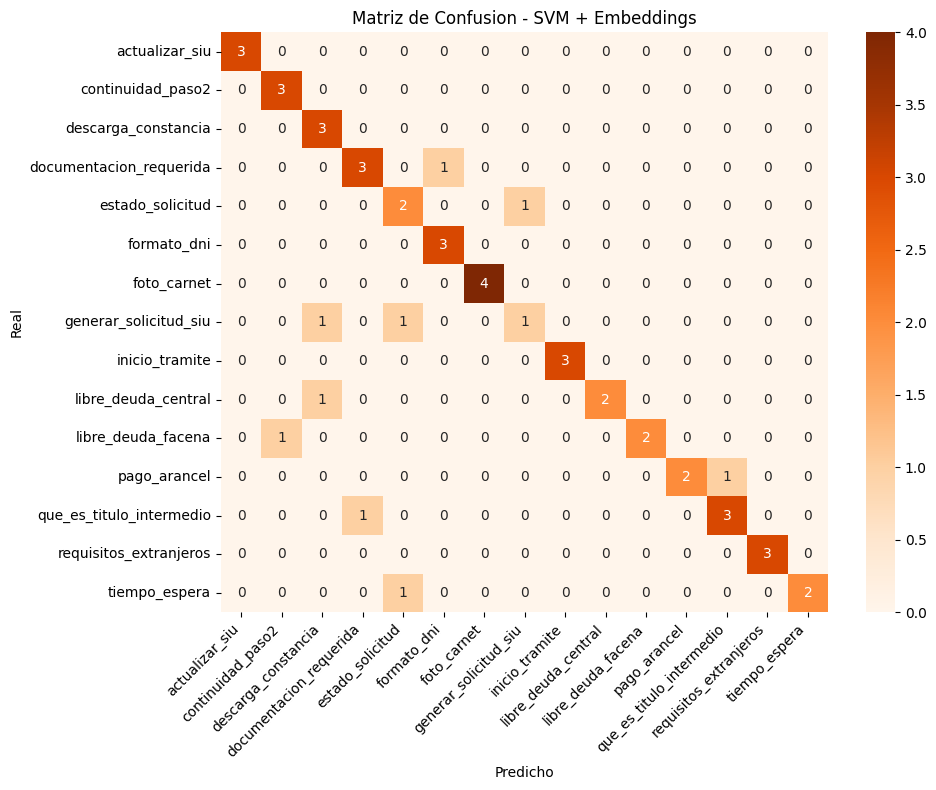
\includegraphics[width=0.30\textwidth]{img/confusion_emb.png}
\caption{Matrices de confusi\'on. Izquierda: NB+TF-IDF ($\alpha=0.5$). 
Centro: SVM Lineal+TF-IDF ($C=1.0$). Derecha: SVM RBF+Embeddings 
($C=10.0$, $\gamma$=scale).}
\label{fig:confusion}
\end{figure*}

\section{Conclusiones}

\subsection{Hallazgos}

\begin{enumerate}
    \item Los embeddings sem\'anticos con SVM RBF superan a TF-IDF, 
          alcanzando 81.25\% de exactitud y 0.81 de F1-macro.
    \item El stemming beneficia a NB (+2\%) pero perjudica a embeddings 
          ($-12.5$ pp), por lo que se descart\'o del pipeline final.
    \item Con datasets peque\~nos (240 muestras), los unigramas son 
          preferibles a bigramas por su menor dispersi\'on.
    \item GridSearchCV identific\'o configuraciones \'optimas con mejoras 
          de hasta 4 puntos respecto a valores por defecto.
\end{enumerate}

\subsection{Trabajos Futuros}

\begin{itemize}
    \item Expansi\'on del dataset a 50+ preguntas por intenci\'on (750+ 
          total) para mejorar la robustez del clasificador.
    \item Incorporaci\'on de t\'ecnicas de data augmentation y balanceo 
          de clases.
    \item Integraci\'on con sistema de ticketing institucional para 
          derivaci\'on de consultas no resueltas.
    \item Evaluaci\'on de modelos de lenguaje pre-entrenados (BERT, GPT) 
          para clasificaci\'on few-shot.
    \item Expansi\'on a otros tr\'amites institucionales.
\end{itemize}

\begin{thebibliography}{00}

\bibitem{raschka2019} S. Raschka y V. Mirjalili, \emph{Python Machine 
Learning}, 3ra ed. Birmingham: Packt Publishing, 2019.

\bibitem{sklearn} F. Pedregosa \emph{et al.}, ``Scikit-learn: Machine 
Learning in Python,'' \emph{JMLR}, vol.~12, pp.~2825--2830, 2011.

\bibitem{sentencebert} N. Reimers e I. Gurevych, ``Sentence-BERT: 
Sentence Embeddings using Siamese BERT-Networks,'' en \emph{Proc. 
EMNLP-IJCNLP}, 2019, pp.~3982--3992.

\bibitem{svm} C. Cortes y V. Vapnik, ``Support-vector networks,'' 
\emph{Machine Learning}, vol.~20, no.~3, pp.~273--297, 1995.

\bibitem{unne} Resoluci\'on RES-2025-7936-REC-UNNE. UNNE. Disponible: 
\url{https://exa.unne.edu.ar/r/?page_id=9008}

\end{thebibliography}

\end{document}
